\section{CERT \& CSIRT}
Heisst: \textbf{Computer Emergency Response Team}\\
Das CERT ist eine Gruppe von IT-Sicherheitsfachleuten, die sowohl präventive als auch reaktive Maßnahmen bei sicherheitsrelevanten Vorfällen in Computer-Systemen empfiehlt.
Sie wirken an der Lösung von konkreten Sicherheitsvorfällen mit, liefern Lösungsansätze oder warnen vor Sicherheitslücken.
Eine andere Bezeichnung für Computer Emergency Response Team ist CSIRT (Computer Security Incident Response Team).
\begin{itemize}
  \item Trademark
  \item Unpräzise
\end{itemize}

Heisst: \textbf{Computer Emergency Security Incident Response Team}\\
\begin{itemize}
  \item Präziser
  \item Free to use
  \item 19 Teams in CH
\end{itemize}

\subsection{Was machen CSIRTs}
Ein CSIRT ist ein Team von IT-Sicherheitsexperten, dessen Hauptaufgabe darin besteht, auf Computersicherheitsvorfälle zu reagieren. 
Es bietet die notwendigen Dienstleistungen an, um diese zu bearbeiten und die Betroffenen bei der Wiederherstellung nach Verstössen zu unterstützen.
Zu den wichtigsten Aufgaben eines CSIRT gehören:
\begin{itemize}
  \item Erstellung und Pflege eines Incident Response Plans (IRP)
  \item Untersuchung und Analyse von Incidents
  \item Verwaltung der internen Kommunikation und Aktualisierung während oder unmittelbar nach Incidents
  \item Kommunikation mit Mitarbeitern, Aktionären, Kunden und der Presse über Incidents nach Bedarf
  \item Behebung von Incidents
  \item Empfehlung von Änderungen in den Bereichen Technologie, Richtlinien, Unternehmensführung und Schulung nach Securityincidents
\end{itemize}

Insgesamt analysiert ein CSIRT die Daten von Incidents, diskutiert Beobachtungen und gibt Informationen im gesamten Unternehmen weiter.


\subsection{SOC}
Der Aufgabenbereich eines SOC kann sowohl Incident Response (ganz oder teilweise) als auch andere Aufgaben umfassen, z.B.:

\begin{itemize}
    \item Überwachung von Abläufen und Kontrollen (z.B. Intrusion Detection / Intrusion Prevention System, etc.)
    \item die Auswertung von Betriebs- und Sicherheitstelemetrie und Informationserfassung beaufsichtigen
    \item Verwaltung von Aufgaben wie Identitätsmanagement und Autorisierung, Wartung von Firewall- und Filterregeln (sowohl Überprüfung als auch Änderungsverwaltung)
    \item forensische und investigative Unterstützung oder andere Aspekte der operativen Sicherheit.
\end{itemize}

\begin{center}
    \vspace{-8pt}
    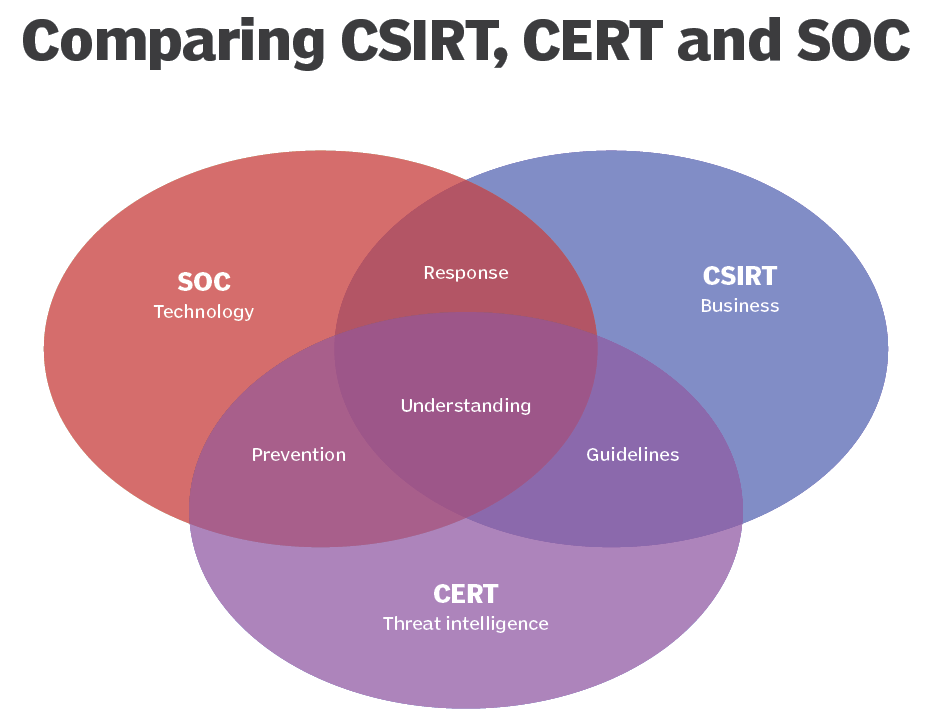
\includegraphics[width=0.8\linewidth]{./img/02-begriffe/soc_cert_csirt}
    \vspace{-8pt}
\end{center}

\subsection{IOC: Indices of Compromize}
Indicators of Compromise (IOCs) definieren die Merkmale eines Vorfalls auf strukturierte Weise. Sie haben das Ziel, Artefakte im Zusammenhang mit Vorfällen zu beschreiben und zu finden.
\textbf{Format:}
\begin{itemize}
    \item Host-basierte IOC-Formate (noch kein akzeptierter Standard)
    \begin{itemize}
        \item YARA
        \item STIX, TAXII
        \item Mandiant's OpenIOX
    \end{itemize}
    \item Netzbasierte IOC-Formate
    \begin{itemize}
        \item Snort rules
    \end{itemize}
\end{itemize}



\subsection{NIST vs. SANS}
\begin{center}
    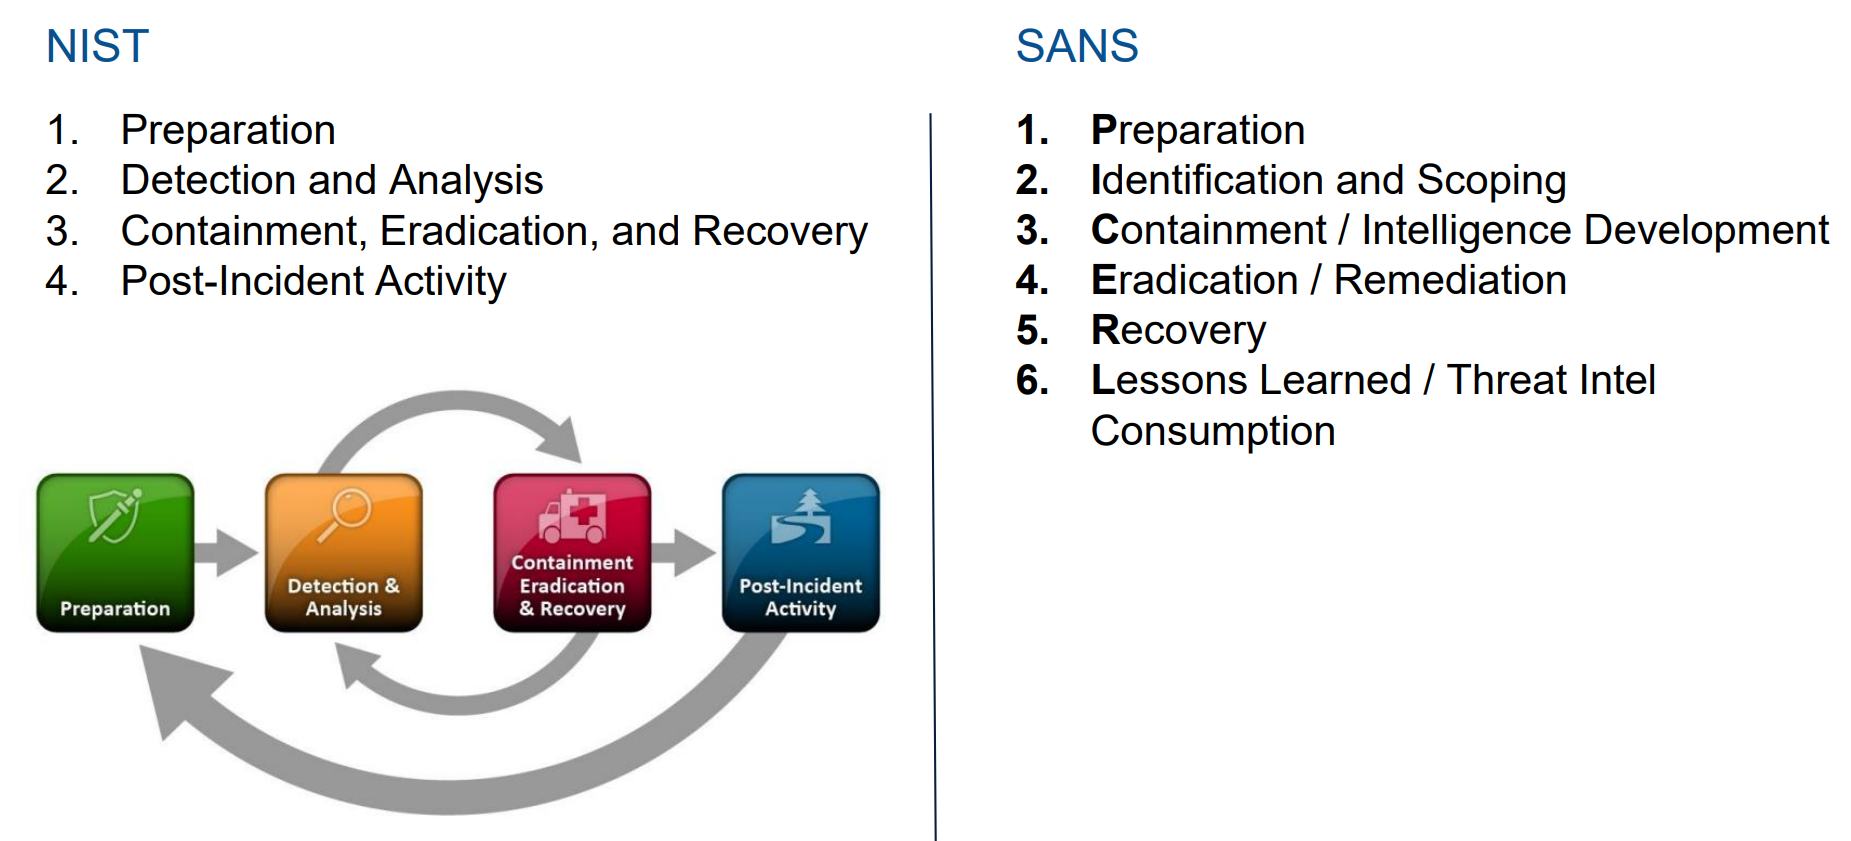
\includegraphics[width=1.0\linewidth]{./img/02-begriffe/nist_sans}
\end{center}